A typical workflow of a scientist who writes a scientific publication is to use a \gls*{wp} to write the publication and one or more \gls*{cas} for Verification, Analysis and Visualization, among other tasks. Especially in \gls*{stem}, \LaTeX\footnote{Note that technically \LaTeX{} is not a \gls*{wp} (\url{https://www.latex-project.org/about/}, seen 07/2017) like \textit{Microsoft Word}. However, since \LaTeX{} (an extension of \TeX) is the standard to write in \gls*{stem} and we only focus on mathematical writings in this thesis, we categorize \LaTeX{} as a \gls*{wp} as well.} has become the de facto standard for writing scientific publications over the last 30 years~\parencites{LATEX:Standard}[559]{DigitalTypo}{Knuth}. \LaTeX{} enables printing of mathematical formulae in a structure similar to handwritten style. For example, consider a Jacobi polynomial~\parencite[18.3 in table 1]{NIST:DLMF}
\begin{equation}\label{eq:P}
P_n^{(\alpha , \beta)}(\cos(a\Theta)).
\end{equation}
This formula is written in \LaTeX{} as
\begin{equation}\label{eq:P-tex}
\verb|P_n^{(\alpha,\beta)}(\cos(a\Theta))|.
\end{equation}

While \LaTeX{} focuses on displaying mathematics, \gls*{cas} focus on computations and user friendly syntax. Therefore, each system (such as \LaTeX{}, \Maple{} or \Mathematica) uses its own representation and syntax. Hence, a writer needs to constantly translate mathematical expressions from one representation to another and back again. Table~\ref{tab:JacobiP-usecase} shows four different representations for the same formula~(\ref{eq:P}).

\begin{table}[ht]
	\centering
	\begin{tabular}{ll}
		\hline
		Systems & Representations \\
		\hline
		\hline
		Generic \LaTeX\ & \verb|P_n^{(\alpha,\beta)}(\cos(a\Theta))| \\ 
		Semantic \LaTeX\ & \verb|\JacobiP{\alpha}{\beta}{n}@{\cos@{a\Theta}}| \\
		\Maple & \verb|JacobiP(n,alpha,beta,cos(a*Theta))| \\ 
		\Mathematica & \verb|JacobiP[n,\[Alpha],\[Beta],Cos[a \[CapitalTheta]]]|\\
		\hline
	\end{tabular}
	\caption{Different representations for the same mathematical formula~(\ref{eq:P}).}
	\label{tab:JacobiP-usecase}
\end{table}

Such translations can become complex, if there are non-obvious differences between the used systems. For example, the \gls*{cas} could use a different order of the arguments, define a normalization of the function for better performances or even use different domains for the variables. Multivalued functions are particularly difficult~\cite{AISC:MultivaluedFunctions}. A \gls*{cas} usually defines so called \textit{branch cuts} to compute principal values of multivalued functions~\cite{Maple:Cuts}. Thereby, implementations of multivalued functions are discontinuous. In general, positioning branch cuts follow some conventions. They are mostly defined conveniently, such as a straight line. However, since a branch cut is a curve, it also can be defined as a spiral or it can be defined for a different position in the complex plane. The position of branch cuts can therefore varies from \gls*{cas} to \gls*{cas}~\cite{Branches:acot}. Figure~\ref{fig:acot-cut-compare} illustrates two examples of different branch cut positioning for the inverse trigonometric arccotangent function. While \Maple{} defines the branch cut at ${[-\infty\iunit, -\iunit]}$, ${[\iunit,\infty\iunit]}$ (figure~\ref{fig:acot-cut1}), \Mathematica{} defines the branch cut at ${[-\iunit, \iunit]}$ (figure~\ref{fig:acot-cut2}).

\begin{figure}[ht]
    \centering
    \subfloat[The real part of arccotangent with a branch cut at ${[-\infty\iunit, -\iunit]}$, ${[\iunit,\infty\iunit]}$.]{%
        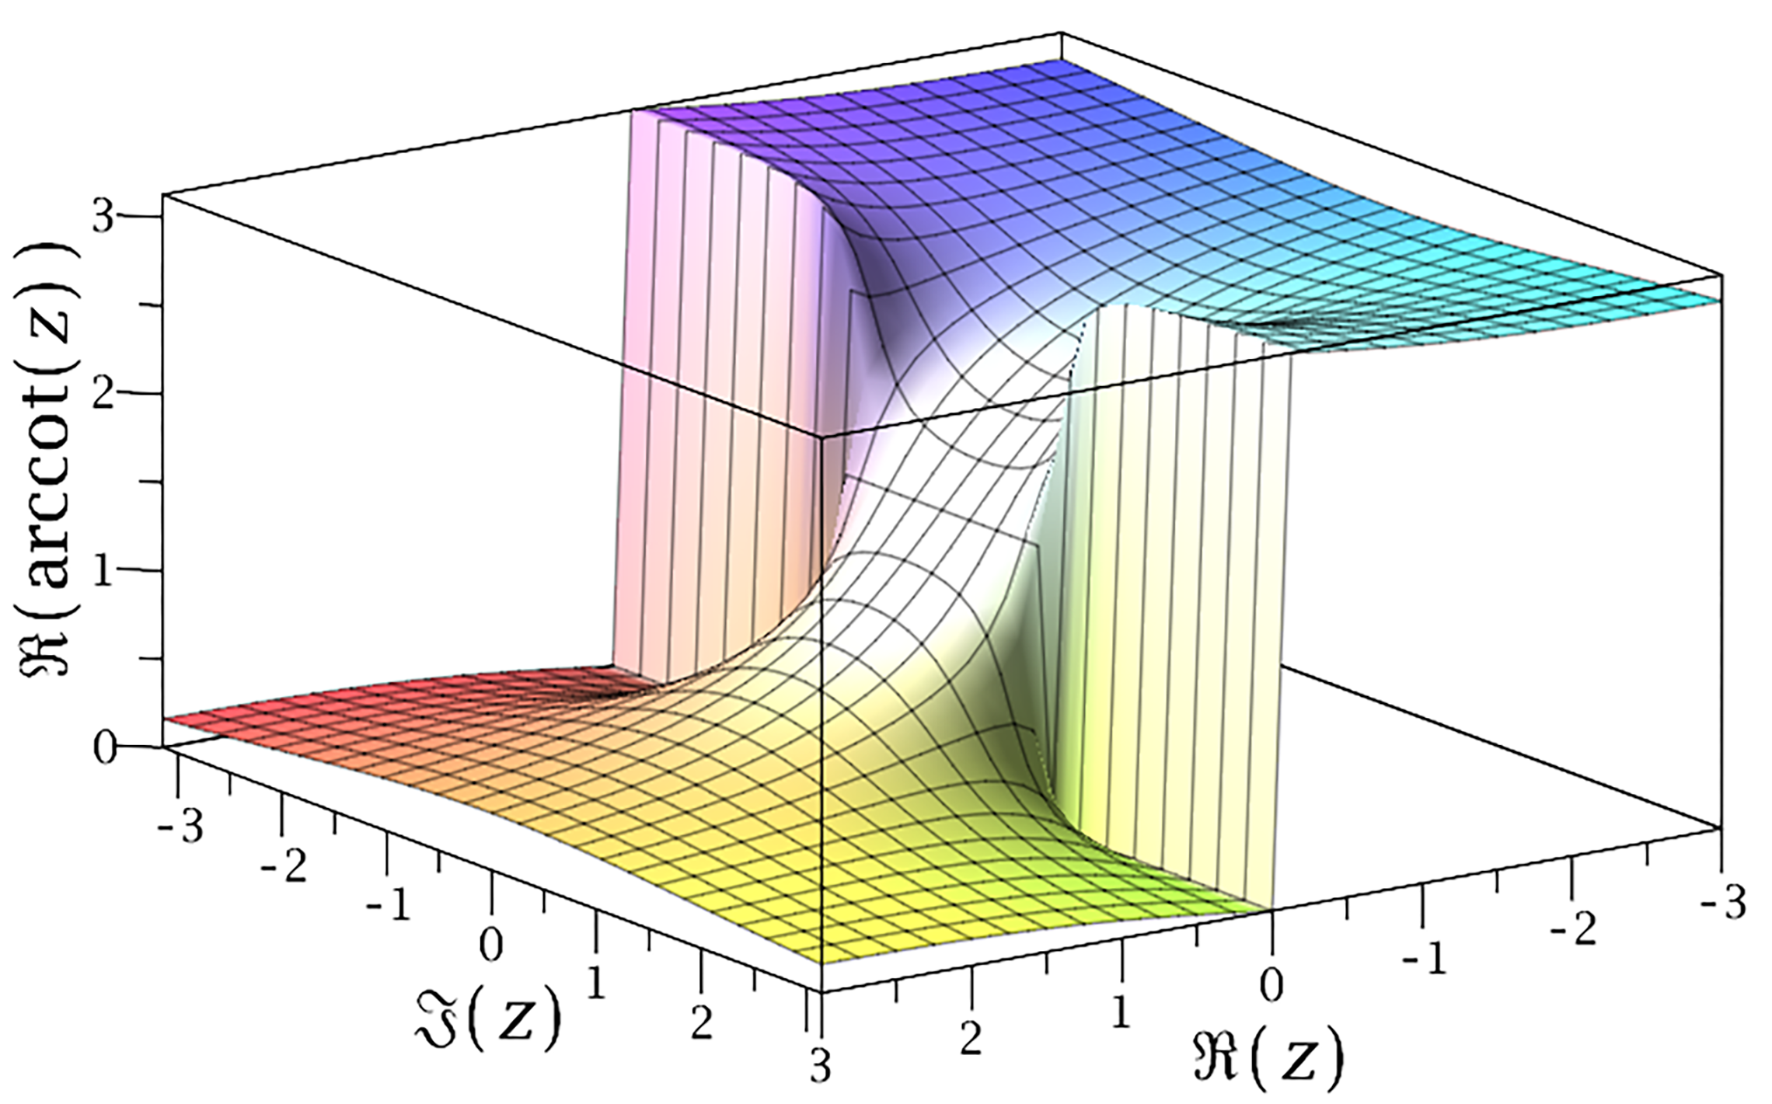
\includegraphics[width=0.45\textwidth]{acotCut1.png}
        \label{fig:acot-cut1}%
    }
    \hspace{0.5cm}
    \subfloat[The real part of arccotangent with a branch cut at ${[-\iunit, \iunit]}$.]{%
        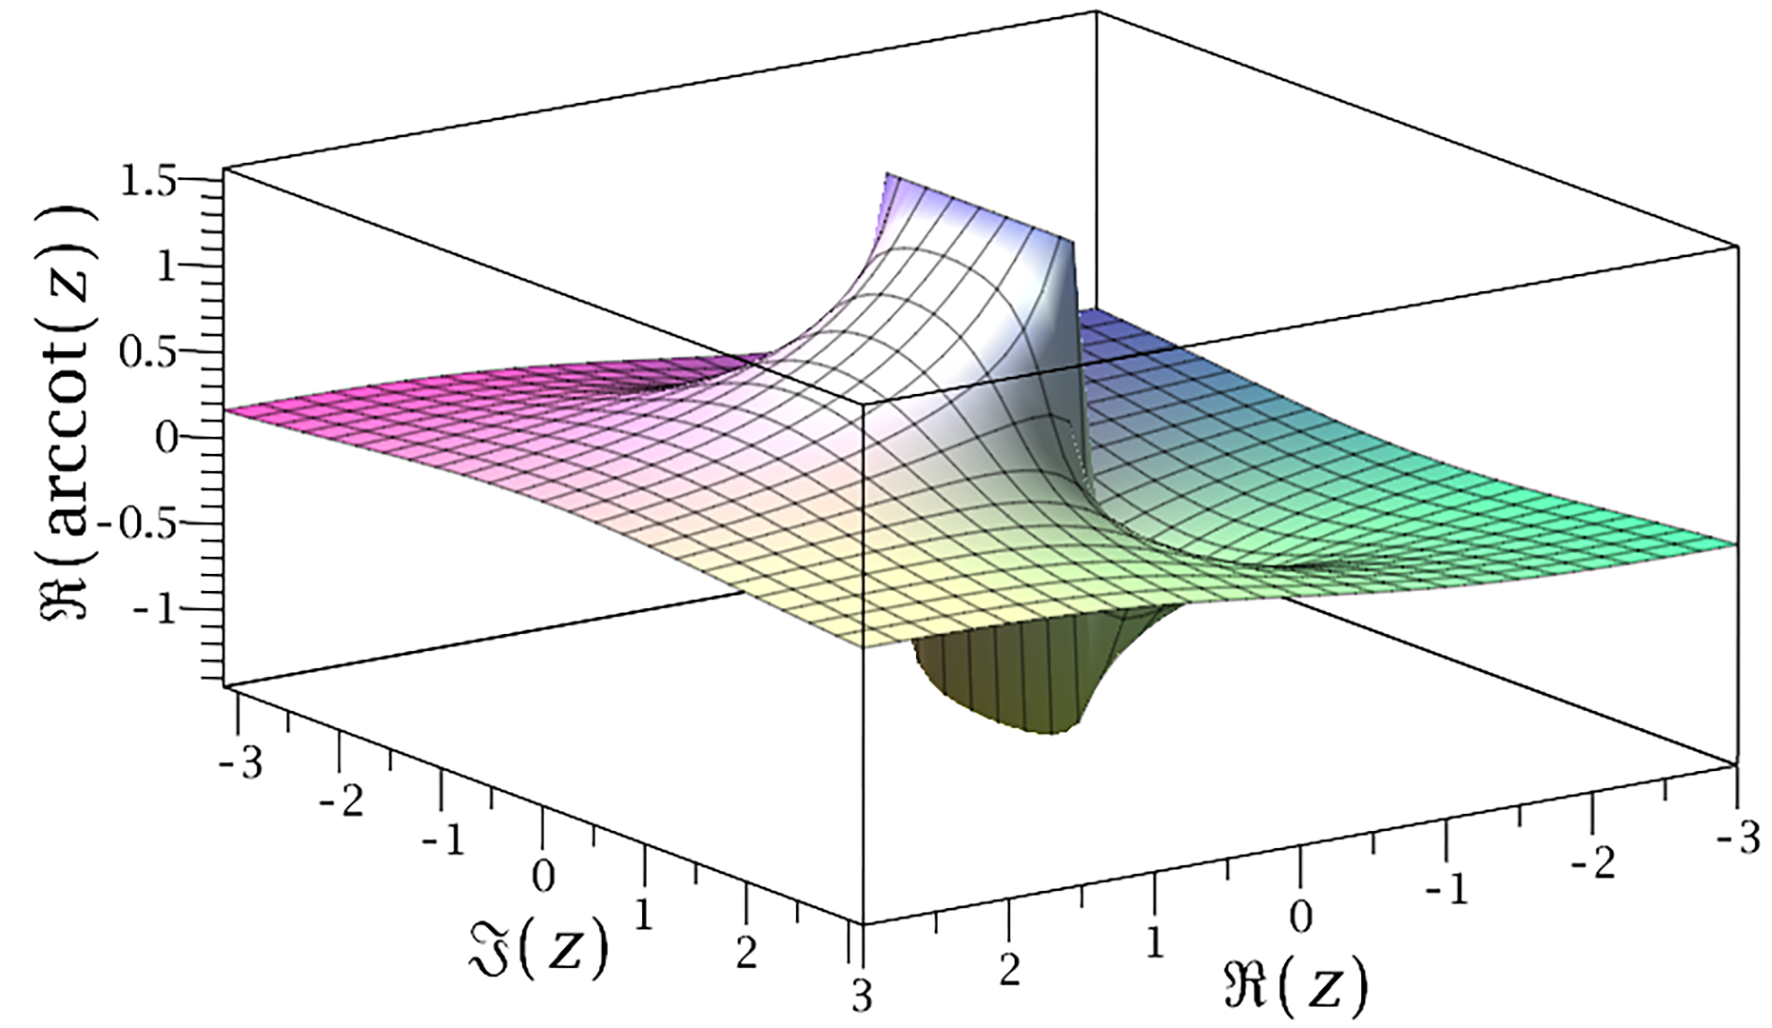
\includegraphics[width=0.45\textwidth]{acotCut2.png}
        \label{fig:acot-cut2}%
    }
    \caption{Two plots for the real part of the arccotangent function with a branch cut at $[-\infty\iunit, -\iunit]$, $[\iunit,\infty\iunit]$ in figure~\protect\subref{fig:acot-cut1} and at $[-\iunit, \iunit]$ in figure~\protect\subref{fig:acot-cut2}, respectively. (Plotted with \Maple{} 2016)}
    \label{fig:acot-cut-compare}
\end{figure}

Hence, a \gls*{cas} user needs to fully understand the properties and special definitions (such as the position of branch cuts) in the \gls*{cas} to avoid mistakes during a translation~\cite{Maple:Cuts}. In consequence, a manual translation process is not only laborious, but also prone to errors. Note that this general problem has been named to automatic \gls*{p2c} conversion~\cite{POM-Tagger}.

An automatic translation process is desirable. Providing translations for mathematical \LaTeX{} expressions is difficult, because the semantic information is absent. Semantics is the meaning of an expression. Consider the example of the Jacobi polynomial in~(\ref{eq:P}). A scientific reader might be able to conclude information like $P$ indicating the Jacobi polynomial and $n$ is being a non-negative integer. However, for a computer it is difficult to understand the expression~(\ref{eq:P-tex}). Since \LaTeX{} is the de facto standard for mathematical expressions, most \gls*{cas} provide import and export functions for \LaTeX{} expressions~\cite{Maple:ImportExport,Mathematica:ImportExport,Matlab:ImportExport,Sage:ImportExport}. However, because of the explained difficulties, those functions are very limited. In fact, they only work for expressions with unique semantic information, but fail for more complex expressions, such as our Jacobi polynomial example.

The \gls*{nist} has therefore developed a set of semantic \LaTeX{} macros~\cite{DLMF:Macros}. Each of these macros is tied with a unique well-defined mathematical object and linked to the corresponding definition in the \gls*{dlmf}~\cite{NIST:DLMF,NIST:DLMF:Paper,NIST:Handbook}. The semantic macros are used to semantically enhance the \gls*{dlmf}. An outgrowth of the \gls*{dlmf} project is the \gls*{drmf}~\cite{DRMF:14,DRMF:15}, which defines more semantic macros, especially for \gls*{opsf}. In table~\ref{tab:JacobiP-usecase} we have already seen an example of a semantic macro. We call \LaTeX{} expressions with semantic macros \textit{semantic \LaTeX{}} and without \textit{generic \LaTeX}, respectively. With semantic \LaTeX, it is possible to provide translations to \gls*{cas}.

Note that partial results of this Master's thesis have already been published at the 10$^\text{th}$ Conference on Intelligent Computer Mathematics 2017~\cite{CICM:Paper}. Techniques, approaches and results have been roughly introduced in the article and are discussed in more detail in this thesis. Pictures and ideas that have already been presented there are not explicitly referenced in the following.

Furthermore, note that the translator we will present in this thesis is based on not published code from the \gls*{mlp} project and the \gls*{pom}-tagger. We will also use the mentioned set of \Macro s, which are not published yet as well. Therefore, the current version of the translator is not online available yet. However, we are planning to publish the translator soon on the \gls*{drmf} website\footnote{\url{http://drmf.wmflabs.org}}.

Moreover, I will use 'we' rather than 'I' in the subsequent chapters of this thesis, since I published and discussed my ideas with others including my advisors Dr.~Moritz Schubotz and Professor Abdou Youssef, the hosts during research visits Howard S.~Cohl and J\"urgen Gerhard, and the students Joon Bang and Kevin Chen.\footnote{Special thanks to M.~Schubotz to give me the permission for using this phrase from his doctoral thesis \cite{MORITZ:Dis}.} 

\section{Goals of the project}
In this thesis, we will present an automatic tool for translations between semantic \LaTeX{} and the \gls*{cas} \Maple{} and \Mathematica. The translation tool should be lite, in a sense that a user does not need a whole software package to use the program. It is also a part of the \gls*{drmf} project and should provide interactive translations in the \gls*{drmf}. Furthermore, it should provide additional information about the translation process and present solutions if an appropriate translation is not possible.

Another goal is the translator's extensibility in order to provide the basis for future work.

\section{Structure}
In the following chapters, we will discuss our translator and verification techniques. Prior to explaining implementation details, we need to introduce some basic background information in chapter~\ref{ch:background}. We start this chapter with an overview of related work (section~\ref{sec:related-work}). Multivalued functions and branch cuts, which were already mentioned, will be introduced in section~\ref{sec:math-background}. Besides the mathematical background, we will discuss semantics in \LaTeX{} in section~\ref{sec:semantics}. A brief introduction to grammar in languages and how we will use it to understand mathematical expressions will be given in section~\ref{sec:mlp}. The chapter is closed by some definitions for the following chapters.

The next chapter~\ref{ch:translator} is the main chapter of the thesis. We will explain implementations and discuss problems and solutions of and for the translator. It starts with an outline of the goals and our approaches in section~\ref{sec:gen-appr}. While we will present implementation details for the forward translations in section~\ref{sec:forward-translation}, we will present the developed backward translation in the following section~\ref{sec:backward-translation}.

In chapter~\ref{ch:evaluation} we will discuss, how we can verify or validate a translated expression. The chapter presents some approaches, such as round trip tests (section~\ref{sec:round-trip}) and numerical tests (section~\ref{sec:numerical-tests}). Extracted formulae from the \gls*{dlmf} and \gls*{drmf} created a comprehensive test suite for these approaches. Section~\ref{sec:test-summary} gives a summary of the results.

The results and the current status of the translation tool will be discussed in chapter~\ref{ch:results}. In conclusion, chapter~\ref{ch:conc-future-work} explains some approaches to further improve the explained techniques in future work.